\setlength{\parindent}{0pt}
\chapter{\bf DISCUSSION}

\gls{dna} replication is a highly conserved and regulated temporal process that is essential to genome inheritance. Yet, stochastic effects of \gls{dna} replication might cause mutagenesis contributing to cancer \citep{tomasetti2015variation}. Therefore, an accurate and properly coordinated \gls{dna} replication is needed to prevent errors and to preserve \gls{dna} fidelity which is constantly threatened by both endogenous and exogenous sources during \gls{dna} replication. Considering 70,000 lesions occur in a single cell per day \citep{lindahl2000repair}, \gls{dna} lesions must be removed before the next cell division, to avoid their permanent conversion into mutations. 

On the other hand, excision repair mechanisms are known to relentlessly coup with \gls{dna} damages that are potential sites of mutations. In deficiencies of mismatch repair and nucleotide excision repair, there are specific mutational signatures contributing to different cancer types \citep{helleday2014mechanisms}. Nucleotide excision repair-associated signature 7 exhibits replication timing differences and replication related strand asymmetry \citep{tomkova2018mutational}. Furthermore, because \gls{erd}s are more reachable relative to \gls{lrd}s, mismatch repair causes a mutagenesis bias between these domains by effectively repairing the mismatches in \gls{erd}s \citep{supek2015differential}. Similarly, \gls{tcr} creates a transcriptional strand asymmetry by repairing adducts only in transcribed strands and leaving the opposite strand untouched \citep{zheng2014transcription}. Even though signature 7 is linked with \gls{dna} replication timing differences and mutational strand asymmetry \citep{tomkova2018mutational}, the contribution of replication to nucleotide excision repair efficiency, and to the resulted mutation distribution is still unclear. In this study, we performed \gls{dsseq} and \gls{xrseq} methods on \gls{uv}-irradiated \gls{hela} cells that are synchronized at early and late S phases to quantify \gls{64} and \gls{CPD} damages and their repair events. 

There are some challenges in measuring the efficiency of nucleotide excision repair during replication. Firstly, because genome is copied once during the replication process, for both early and late S phases, only a fraction of the genome was replicated when the experiments were conducted. Thus, we might observe a weak replication effect on repair rates throughout the genome, even though there is a strong effect in the regions that are replicated. Moreover, bulky \gls{dna} adducts can interrupt replication fork, which initiates inter-S phase checkpoint and therefore, delays the replication \citep{minca2011replication}. Delaying of replication prevents us to successfully locate the exact sites of replication forks, which might reveal the local replication effect on nucleotide excision repair. To overcome these challenges, we focused our analyses only on replication-associated regions such as defined replication domains \citep{liu2016novo}, initiation zones \citep{petryk2016replication}, and replication origins \citep{besnard2012unraveling} of \gls{hela} cells.     

\section{DNA replication elevates nucleotide excision repair rate.}

In the first part of the study, we examined the repair rate of nucleotide excision repair at large regions, while replication moves from early S phase to late S phase. We normalized repair events to damage (repair rate) for 2 reasons; firstly, to eliminate the sequence context bias that can lead to more damage formation, thus more repair. Secondly, \gls{dna} content of replication domains during replication are not even. Because, \gls{erd}s are replicated earlier, it is expected to have more \gls{dna} content from these domains. After calculating the repair rates in replication domains, we found that \gls{erd}s are repaired more efficiently that \gls{lrd}s in both early and late S phases (Figure \ref{fig:repdomain}). Because \gls{erd}s usually correspond to open chromatin sites, they are more reachable for nucleotide excision repair, which in turn, promote efficient repair. This result suggests that, like mismatch repair \citep{supek2015differential}, nucleotide excision repair creates a mutational difference between \gls{erd}s and \gls{lrd}s by efficiently repairing \gls{erd}s. Moreover, replication domains are repaired with better efficiency when they are being replicated, which can be an indirect effect of replication progress by opening closely packed chromatin and thereby, promoting the nucleotide excision repair initiation (Figure \ref{fig:repdomain}). This effect is less prominent for \gls{64} damages than that of \gls{CPD}s, because they are repair faster and less effeted by chromatin states. In addition, \gls{CPD}s at 2 hours exhibits less replication effect than that of \gls{CPD}s at 12 minutes, possibly caused by the occurred \gls{dna} damages that interrupt replication. 

Then, we examined the differences in repair rates of chromatin states for both \gls{erd}s and \gls{lrd}s. The chromatin states that are associated with close regions are more varying in \gls{erd}s, likewise, the chromatin states that are associated with open regions display same phenomenon in \gls{lrd}s, simply because \gls{erd}s have less heterochromatin regions, while \gls{lrd}s have less open regions. Expectedly, the active promoters and enhancers are repaired efficiently for both \gls{erd}s and \gls{lrd}s. Moreover, the major difference between phases occurred on close chromatin states (Figure \ref{fig:chromatin}, \ref{supfig:chromatin1}-\ref{supfig:chromatin5}). This result indicates that movement of replication elevates the repair rates of close chromatin states by mediating chromatin opening. Lastly, we proposed a simple model to deminstrate the replication effect on repair (Figure \ref{fig:model}).     

\begin{figure}[H]
    \begin{center}
    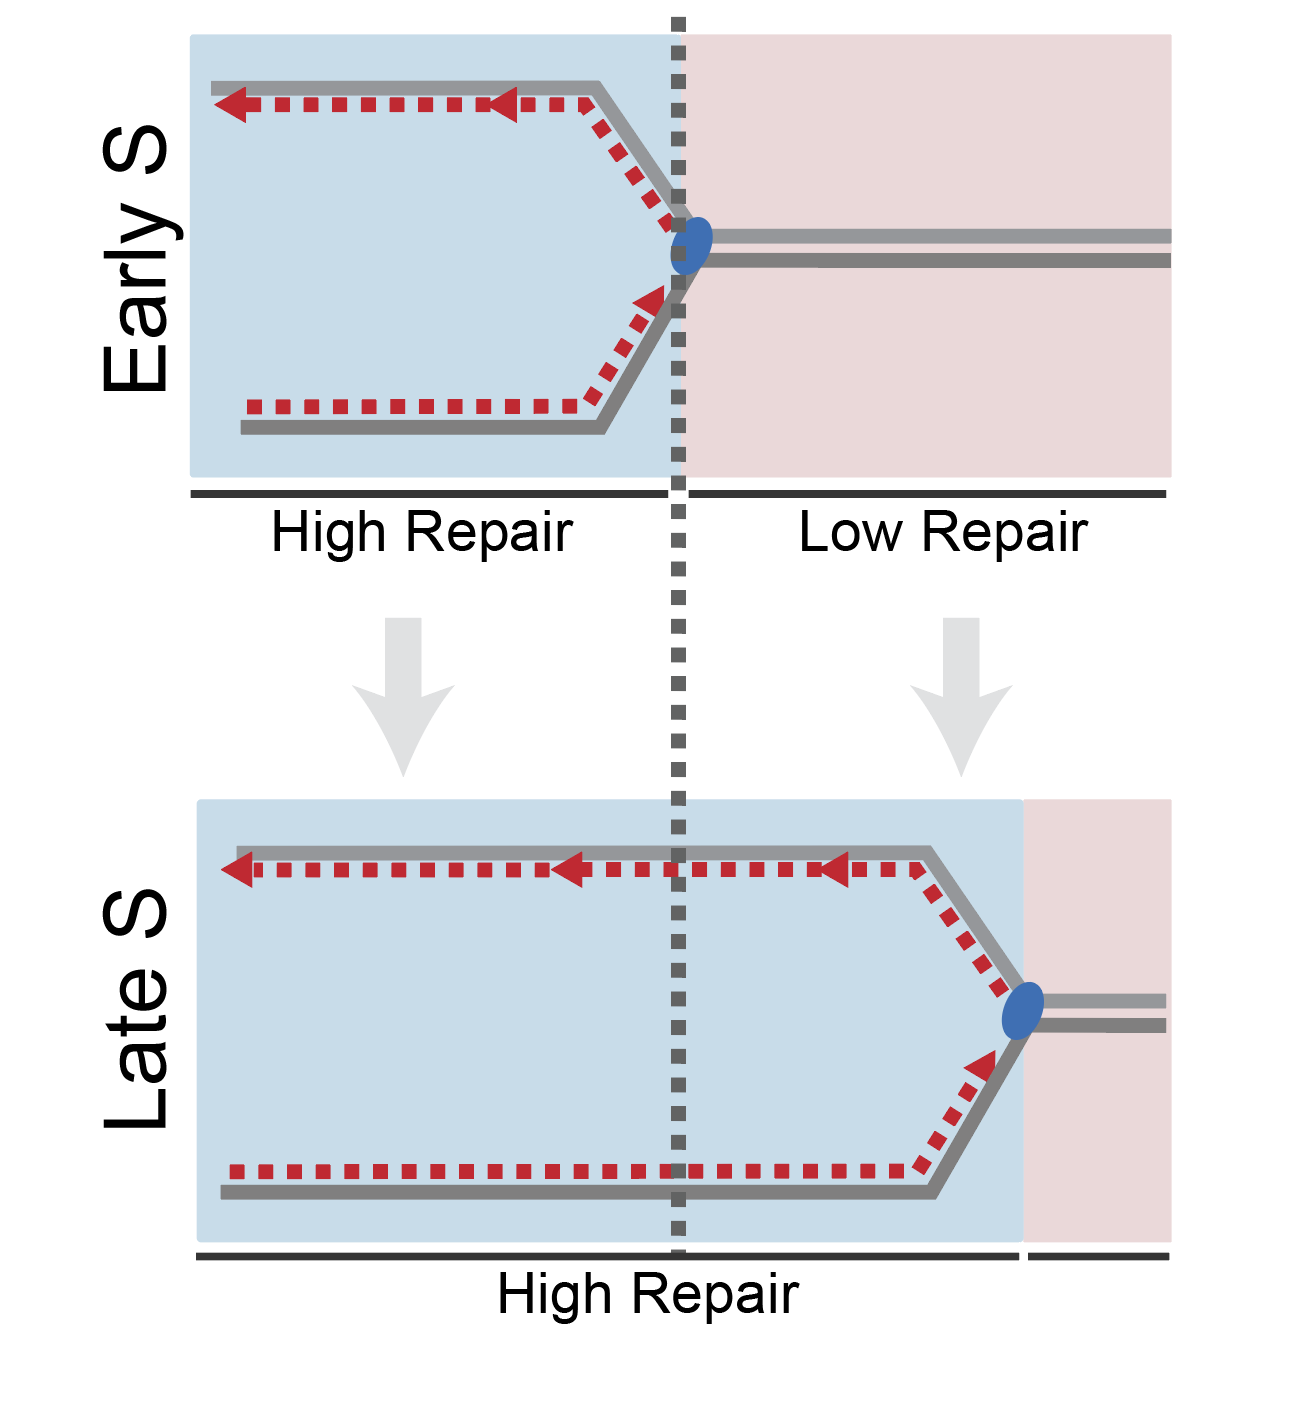
\includegraphics[width=0.8\columnwidth]{Chapters/5_discussion/figures/model}
    \caption[Repair preferences of Nucleotide Excision Repair during replication.]{Repair preferences of Nucleotide Excision Repair during replication. During the early S phase, open chromatin regions (blue) which mostly correspond to \gls{erd}s, are repaired better than the condensed regions (red) because nucleotide excision repair can reach the open chromatin sites more efficiently than it reaches the condensed regions. While replication continues, those condensed regions loosen and become more reachable for excision repair.}
    \label{fig:model}
    \end{center}
    \end{figure}

\section{Mutagenesis, UV-induced DNA damage, and repair display replicational strand asymmetry}

Secondly, we examined a possible replicational strand asymmetry of mutagenesis, \gls{uv}-induced \gls{dna} damage, and repair, respectively. Bidirectional movement of replication forks leads to asymmetric progress of polymerases \gls{epsilon} and \gls{delta}. Considering these polymerases act differently when they are introduced with a lesion, the initiation of nucleotide excision repair might not occur at the same efficiency, thus might create a replicational strand asymmetry. On the lagging strands that are synthesized by polymerase \gls{delta}, replication will not be inhibited when the replication fork encounters a damage, because of the discontinuous synthesis of Okazaki fragments. Instead, small gaps are left opposite to the damage site, which might be repaired post-replicative mechanisms. Conversely on the leading strand, while helicase continues to unwinding double-stranded \gls{dna}, polymerase \gls{epsilon} will be stalled. This disagreement then leads to \gls{ssdna} gaps that induce \gls{atr} pathway, thus increase the chance of repair \citep{byun2005functional}. In fact, multiple studies reported that the leading strands harbors less mutation than the lagging strands in multiple cancers \citep{haradhvala2016mutational,lujan2012mismatch,reijns2015lagging,shinbrot2014exonuclease}. Even though this difference usually associated with replication-related processes such as POLE- and APOBEC-related mutagenesis \citep{haradhvala2016mutational}, we observed a significant mutational strand asymmetry at melanoma cancers, which are related to UV induced damages. 

To assess the contribution of nucleotide excision repair on the mutagenesis, we further mapped damage and repair events on these regions separately. Remarkably, we observed a repair bias towards the leading strands (Figure \ref{fig:mutation}), which is both in aggreament with mutational strand asymmetry of melanoma mutations and results of a recent study \citep{seplyarskiy2019error}. Furthermore, by revealing that both simulated and observed damage and repair events prefer the leading strands (Figure \ref{fig:simulation}), we suggested that the strand asymmetry is somewhat caused by the sequence context. This preference is more prominent on \gls{CPD}s at 2 hours, whereas \gls{64}s and \gls{CPD}s at 12 minutes display a weak or no preference to the leading strands. One possible reason can be that 12 minutes might not be enough to resolve polymerase-blocking at the lesion site. However, the pattern of \gls{CPD} repair at 2 hours indicates the effect of replication on repair. Similarly, \gls{CPD}s at 2 hours on high \gls{rfd} exhibits a 100 to 200 \gls{kb} long repair rate difference towards the leading strands, while \gls{64}s and \gls{CPD}s at 12 minutes display no difference between strands (Figure \ref{supfig:rr20rfdA}-\ref{supfig:rr2000rfdB}). However, \gls{64}s and \gls{CPD}s at 12 minutes around individual replication origins that are defined by \gls{snsseq} data, exhibit a strand asymmetry on repair rate that favor the lagging strands, which is not consistent with other findings (Figure \ref{fig:repairrate}, \ref{supfig:rr200inzonesA}, \ref{supfig:rr200inzonesB}, \ref{supfig:rrpm20inzonesA}-\ref{supfig:rrpm200inzonesB}). In fact, the difference between the repair and damage events are so small that can only be observed in a 5 kb region. Moreover, \gls{CPD}s at 2 hours indicate a strand asymmetry on repair rate that favors the leading strands, which is in aggreament with other findings. Notably, \gls{lrd}s have higher asymmetry of repair rates in both early and late S phases. Even though it is expected to observe this in late S phases, simply because \gls{lrd} repair is elevated when it is replicated (Figure \ref{fig:repairrate}), however, it not expected to observe this phenomenon in early S phase. Considering that replication is a dynamic process that is not fully strict on its order, there can be some initiation of replication forks in \gls{lrd}s, which can create the asymmetry.         

In conclusion, \gls{dna} replication can impact the efficiency of nucleotide excision repair on two levels. At genome-wide scale, \gls{erd}s are repaired faster than \gls{lrd}s in both early and late S phases. Also, by opening the heterochromatins, replication promotes the repair of \gls{lrd}s. In the scale of the replication origins, a replicational strand asymmetry is persistent in multiple replication-associated regions (individual replication origins, initiation zones, high \gls{rfd} regions) and around initiation zones, there is a significant mutational strand asymmetry as well. By the stalling of polymerase \gls{epsilon} during replication, the leading strands are repaired more efficiently than the lagging strands, especially when the time after the \gls{uv} exposure is increased. These findings reveal the contribution of nucleotide excision repair together with replication timing to mutational strand asymmetry of cancer genomes.

